\documentclass[10pt,a4paper]{article}
\usepackage[margin=2.2cm]{geometry}
\usepackage{amsmath,amssymb}
\usepackage{booktabs,graphicx,xcolor,enumitem,caption}
\usepackage[hidelinks]{hyperref}
\usepackage{float}
\captionsetup{font=small}
\setlength{\parskip}{3pt}
\newcommand{\pend}[1]{\textcolor{red}{\textbf{[#1]}}}
\newsavebox{\claimsave}
\newenvironment{claimbox}[1]{\begin{lrbox}{\claimsave}\begin{minipage}{0.94\linewidth}\textbf{#1}\par\vspace{2pt}}{\end{minipage}\end{lrbox}\begin{center}\setlength{\fboxsep}{6pt}\fcolorbox{blue!50!black}{blue!4}{\usebox{\claimsave}}\end{center}}

\title{\textbf{Structure-Aware Drafting for Generative UI:\\Choosing Where to Copy From, Using the Shape of HTML}}
\author{GenerativeUI project, KSEF26 --- research claim note, English version}
\date{2026-11-07}
\begin{document}
\maketitle

\begin{claimbox}{Claims}
\begin{enumerate}[leftmargin=1.4em,itemsep=2pt]
\item By combining known techniques, giving the model similar example screens and letting it reuse pieces of them as drafts, a small model builds a screen about 11 times faster with no loss in accuracy. Half of the screen appears after 3.3 seconds instead of 48.2 seconds.
\item The remaining waste is in \emph{where} the drafts are copied from. HTML repeats the same short pieces many times, so the usual method often continues from the wrong place.
\item A simple rule that follows the structure of the HTML picks better places and cuts model steps by 7.9\%, more than general-purpose improvements. Picking the best place every time would cut steps by a factor of 1.76, so there is a lot of room for a learned chooser.
\item We also tried learning which examples give the fastest answer and accepting drafts that give the same screen. Both were honest dead ends: the gains were small or could not be predicted.
\end{enumerate}
\end{claimbox}

\section{The problem}
In \emph{generative UI}, a user types a request such as ``a login screen with a Sign up button'', and a language model writes the HTML code for that screen. HTML is the language web pages are written in; CSS is the part of it that sets colors, sizes and positions. The browser draws the code as a picture, and the user only ever looks at that picture.

The model writes code one small piece at a time. Each piece is a \emph{token}, roughly a short word or a few characters, and each token costs one full step of the model. So
\begin{equation}
\text{waiting time} \;\approx\; \text{number of model steps} \times \text{time for one step}.
\end{equation}
In words: to make the user wait less, we must make the model take fewer steps. With normal generation there is one step per token, so a screen of 1000 tokens needs 1000 steps.

We use Gemma~4, a family of freely available language models from Google. Most results use the smallest one, named E2B, which we simply call the small model. Without help it takes about a minute per screen.

\section*{Part 1. What we confirmed}

\section{The system works: about 11 times faster with the same accuracy}
Two known ideas do most of the work.
\begin{itemize}[itemsep=1pt]
\item \textbf{Give examples.} We put three existing screens that look like the answer into the request. The model then copies a lot and writes shorter code.
\item \textbf{Reuse the examples as drafts.} Instead of one token per step, we take the next several tokens from an example as a guess, called a \emph{draft}, and let the model check the whole draft in a single step. Checking many tokens costs about the same as writing one. The model keeps the part it agrees with, so its output does not change.
\end{itemize}
The speed-up from drafting is roughly
\begin{equation}
\text{times faster} \;\approx\; \text{average number of tokens the model accepts per step}.
\end{equation}
In words: if the model accepts 5 tokens per step instead of 1, generation is about 5 times faster.

\begin{table}[H]\centering\small
\caption{Small model, 10 test screens, medians. ``Times faster'' compares with the first row. Sources: \texttt{runs/poc/E2B\_Ctable.md}, \texttt{runs/poc/E2B\_perc.md}.}\label{tab:main}
\begin{tabular}{lrrrcc}
\toprule
method & whole screen & half visible & times faster & checklist & element match\\
\midrule
no examples, normal & 59.4 s & 48.2 s & 1.0 & 87\% & 48\%\\
word examples, normal & 27.1 s & 20.3 s & 2.2 & 100\% & 50\%\\
word examples, drafts & 6.6 s & 4.5 s & 9.0 & 100\% & 50\%\\
layout examples, drafts & 5.3 s & 3.3 s & \textbf{11.2} & 100\% & 51\%\\
\bottomrule
\end{tabular}
\end{table}

The \emph{checklist} is our main accuracy score: the request names two to four elements, such as ``a Cancel button'', and we check whether each one appears on the generated screen. The \emph{element match} compares the elements of the generated screen with the true screen. Both stay the same or improve. We stress that this result is a combination of existing techniques; it is the starting point, not our new contribution.

\section{Searching examples by layout keeps the speed and meets more requests}
Ordinary search finds examples whose words match the request. We trained a simple model that predicts the \emph{layout} of the answer screen from the request, for example ``a top bar, a list, two buttons at the bottom'', and picked the existing screen with the closest layout.
\begin{itemize}[itemsep=1pt]
\item On 50 screens with drafting, layout-search examples raised the checklist from 94.8\% to 98.2\%. The gain is 3.3 points, and its 95\% confidence interval runs from 0.2 to 7.2 points, so it is unlikely to be luck. The time stayed the same: 5.6 versus 5.7 seconds.
\item But if we simply copy the top example as the answer without a model, layout search does \emph{worse} on the checklist, by 8.3 points on 100 development screens. Layout examples help the model, not a copy machine.
\end{itemize}

\section{Examples with more copyable code are not faster, and the fastest example is hard to predict}
We expected that the example sharing the most code with the true answer would be the fastest. It was the opposite: choosing by largest shared code made each screen 1.40 seconds slower, with a 95\% confidence interval of 0.41 to 2.42 seconds. Those examples tend to be longer.

Next we ran six different example choices for each of 50 requests and timed all of them.
\begin{itemize}[itemsep=1pt]
\item The choice matters a lot. The top word-search example took 9.33 seconds on average, while the fastest of the six took 4.73 seconds, 37\% less.
\item Three quarters of this difference comes from how long the model's answer is, and one quarter from how many drafts it accepts.
\item But nothing we can know before generating predicts it well: every such signal had a correlation of 0.13 or less with the time. A correlation is a number from $-1$ to $1$ that says how strongly two things move together.
\item A learned chooser closed only 13\% of the gap, and that gain was not statistically clear.
\end{itemize}
So we do not claim learning fast examples as a contribution.

\section{Two smaller ideas with limited effect}
\paragraph{Accepting drafts that give the same screen.} Different code can draw the same screen; for example \texttt{<p>Hello</p>} and \texttt{<p>Hello} look identical. We tried accepting a draft whenever it gives the same screen, even if the code differs. But only 6\% to 18\% of rejected drafts turned out to give the same screen, so the room for this idea is small.

\paragraph{Changing the order of style code.} The model normally writes all the style code first, so the screen stays blank for a long time. Moving each style rule to just before the part it styles keeps the final screen identical. With normal generation this helped: half the screen appeared at 67\% of the run instead of 81\%. With drafts it did not help: half the screen appeared after 4.0 seconds instead of 3.5 seconds.

\section*{Part 2. Our proposal: structure-aware choice of where to draft from}

\section{The problem: HTML repeats itself}
To make a draft, the usual method looks at the last few tokens the model wrote, searches for the same tokens in the examples, and copies what follows. In HTML the same short pieces, such as \texttt{"><div class="}, appear many times inside one example. The method then often jumps to the wrong copy and continues from the wrong place, and the model rejects the draft.

We can state the choice as
\begin{equation}
\text{best place} \;=\; \text{the place in the examples whose continuation the model will accept the most tokens of}.
\end{equation}
In words: among all places in the examples where we could start copying, we want the one that leads to the longest accepted draft. The usual method just takes the most recent text match.

\section{Evidence}
We replay the outputs we already have and count how many model steps each way of choosing the place would need. This counts accepted tokens under ideal normal generation; it does not measure real time.
\begin{enumerate}[itemsep=1pt]
\item \textbf{The replay is faithful.} For the usual method, it reproduces the number of model steps in our real logs on 10 of 10 screens.
\item \textbf{Choosing the place is a large lever.} If we always picked the best place, the model would need 1.76 times fewer steps. In 46\% of the steps where the usual method accepted almost nothing, another place in the examples would have given two or more accepted tokens.
\item \textbf{HTML structure beats general fixes.} A rule that also checks where we are in the HTML structure, for example ``we just closed an element, so continue with the next element in the example'', cuts steps by 7.9\%, with a 95\% confidence interval of 6.4\% to 9.5\%. Matching longer text cuts only 4.0\%, and voting among several matches only 0.7\%. Compared request by request with the best general fix, the structure rule saves 4.4 to 8.9 steps per screen at 95\% confidence. About 60\% of its extra accepted tokens come from the points where one element ends and the next begins.
\item \textbf{There is room to learn.} Even with the rule, 81\% to 85\% of the gap to the best possible place remains.
\end{enumerate}

\begin{figure}[H]\centering
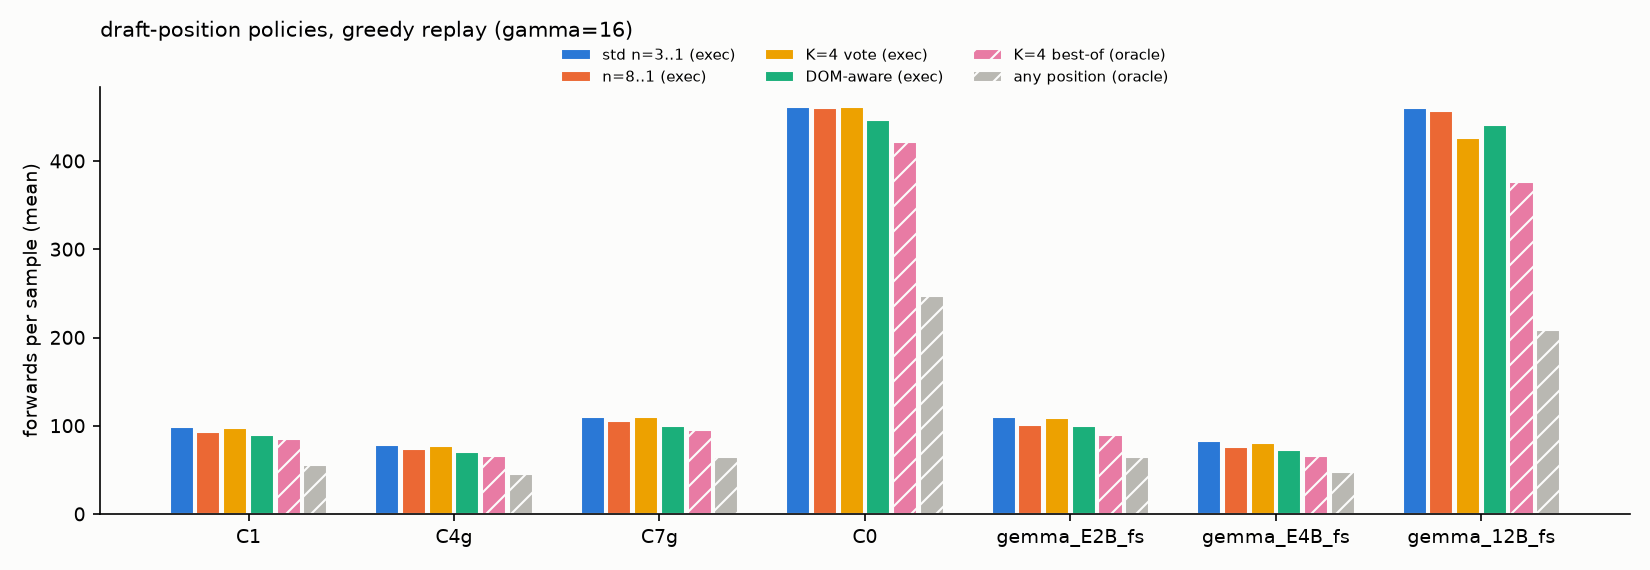
\includegraphics[width=\linewidth]{../runs/study/figures/draft_sim.png}
\caption{Model steps per screen, lower is better, for each way of choosing the draft place. In each group, blue is the usual method, green is our structure rule, and grey is the best possible place. The four left groups are the small model with different examples; the three right groups are the small, medium and large Gemma~4 models.}\label{fig:sim}
\end{figure}

\section{Proposed contribution}
\begin{enumerate}[itemsep=1pt]
\item \textbf{Problem.} We show that because HTML repeats itself, text-matching drafts often start from the wrong place, and that this is where most of the remaining waste lies.
\item \textbf{Learning.} We build a place chooser that predicts how many tokens will be accepted from each place, using where we are in the HTML structure and the model's own internal state.
\item \textbf{Use.} The model still checks every draft exactly as before, so the output does not change. Only the choice of draft changes.
\end{enumerate}

\paragraph{Next steps.} Improve the learned chooser by telling it whether a place continues the previous draft, training it to rank places rather than to guess counts, and training it on its own real runs; measure real time on the graphics card; and find out why the gain disappears for the larger model.

\section{How we test}
Our test set is built from Screen2Words, a public collection of about 22{,}000 real Android app screens with five human descriptions each. Each item is a request plus the true screen as HTML. The request gives the purpose and two to four key elements, but not counts or long text, so many different screens are correct. The true screens pass 100\% of their checklists; a fixed template passes 8\%, and copying the most similar existing screen passes 37\%. We use 500 test screens, 100 development screens and 14{,}522 example screens, with no app shared between these groups.

\section{Limitations}
\begin{itemize}[itemsep=1pt]
\item Speed was measured on 10 to 50 screens. On 10 screens the checklist is almost always 100\%, so it barely separates methods.
\item Drafting should not change the output, but rounding in 4-bit and 16-bit arithmetic made 7 of 10 outputs differ slightly from normal generation. The model also runs in a 4-bit format that only approximates the official one.
\item The structure rule was clearly better only for the small model on our main, medium-detail requests. With detailed requests and the larger model, its advantage was not statistically clear.
\item Our first learned place chooser is still worse than the simple rule: 6.6\% fewer steps against 7.9\%.
\item The place-choice results count model steps in a replay; real time has not been measured yet.
\end{itemize}

\end{document}
